\documentclass[11pt,letterpaper,landscape,openany]{scrbook}\renewcommand{\familydefault}{\sfdefault}\usepackage{cjhebrew}\usepackage{tabularx}\usepackage[letterpaper,bindingoffset=0.2in,left=1in,right=1in,top=.5in,bottom=.5in,footskip=.25in,marginparwidth=5em]{geometry}\usepackage{marginnote}\usepackage{graphicx}\usepackage{wasysym}\usepackage{sectsty}\usepackage{xcolor}\definecolor{hcolor}{HTML}{D3230C}\newcommand{\red}[1]{\textcolor{hcolor}{#1}}\setkomafont{disposition}{\bfseries}\newcommand\Chapter[2]{\chapter[\normalfont#1:{\itshape#2}]{#1\\[1ex]\Large\normalfont#2}}\makeatletter\newcommand{\alephbet}[1]{\c@alephbet{#1}}\newcommand{\c@alephbet}[1]{{\ifcase\number\value{#1}\or\<'>\or\<b>\or\<g>\or\<d>\or\<h>\or\<w>\or\<z>\or\<.h>\or\<.t>\or\<y>\or\<k|>\or\<l>\or\<m|>\or\<n|>\o\<N>\or\<s>\or\<`>\or\<p|>\or\<P>\or\<.s>\or\<q>\or\<r>\or\</s>\or\<t>\fi}}\renewcommand{\partname}{}\renewcommand\thepart{\alephbet{part}}\renewcommand\thechapter{\alephbet{chapter}}\allsectionsfont{\centering}\newcolumntype{Y}{>{\centering\arraybackslash}X}\begin{document}\noindent\large I made this calendar because, after scouring the Internet, I couldn't find any calendars at all for Aquatic Judaism. Accordingly, I thought that it might be educational to make a such a calendar for Terrestrial Jews who might not be familiar with Aquatic Judaism. \newline\newline Besides some difference in which yom tovs to observe, and how to observe them, the single greatest difference between the Terrestrial and Aquatic Jewish calendar is how days are measured. The secular (Gregorian) calendar is \textit{solar}: days, months, and years are based on the Earth's movement around the Sun. The Terrestrial Jewish calendar is \textit{lunisolar}: Days are based on the Earth's movement around the Sun, while months and years are based on the phases of the Moon. The Aquatic Jewish calendar is \textit{lunitidal}: Days are based on the local high tides, while months and years are based on the phases of the Moon. \newline\newline Aquatic Judaism varies by region and denomination in a manner similar to Terrestrial Judaism, but the boundaries between the groups are looser, as befits a people that lives beyond national borders. The notes I've included in this calendar are mostly for Atlantic Aquatic Judaism, which is roughly analogous to Terrestrial Ashkenazi Judaism. \newline\newline The sinusoidal waves on this calendar are based on NOAA preliminary data. For most observant Aquatic Jews, this is insufficiently accurate. For one, the charts here are based on predictions specifically for Boston, Massachusetts, and will vary the further out one is from Boston Harbor. For another, none can truly predict the tides, which are determined ultimately by God's will alone. It is customary in more traditional flotillas to measure the tides only on the day-of, and to blow a shofar at each high tide.\newpage There will be an image here.\normalsize\chapter*{Tishrei}\noindent\begin{tabularx}{\textwidth}{YYYYYYY}\normalsize Dag&\normalsize Gal&\normalsize Khof&\normalsize Sa'ar&\normalsize Shakhaf&\normalsize Melakh&\normalsize Shabbat\\\end{tabularx}\\\noindent\begin{tabularx}{\textwidth}{|X|X|X|X|X|X|X|}\hline{\huge\textbf{1\rule{0pt}{2ex}}  \hfill \CIRCLE}\newline {\tiny{09.09.18 03:00 AM}}\newline\scriptsize{\textbf{Rosh Hashanah\marginnote{\tiny{\textbf{Rosh Hashanah}\newline\textit{Tashlikh must be performed in a salty body of water.}}}}}\newline 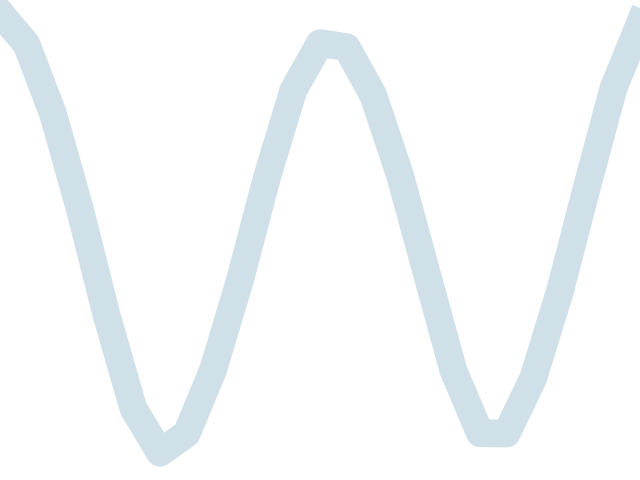
\includegraphics[width=\linewidth,keepaspectratio=true]{plots/0.png}&{\huge\textbf{2}  \hfill }\newline {\tiny{09.10.18 04:00 AM}}\newline\scriptsize{\textbf{Rosh Hashanah}}\newline 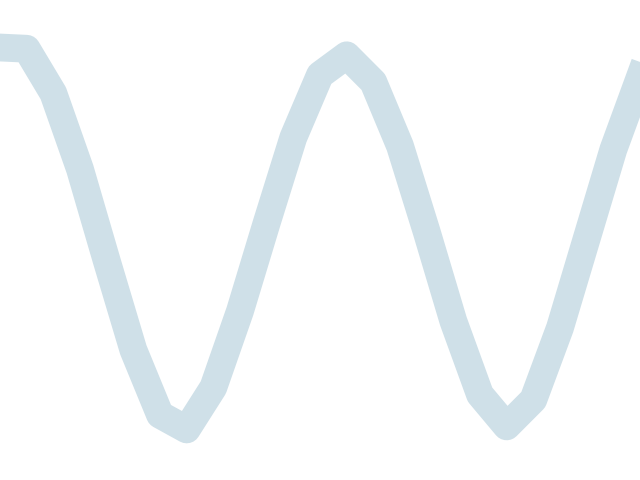
\includegraphics[width=\linewidth,keepaspectratio=true]{plots/1.png}&{\huge\textbf{3}  \hfill }\newline {\tiny{09.11.18 05:00 AM}}\newline\scriptsize{\textbf{}}\newline 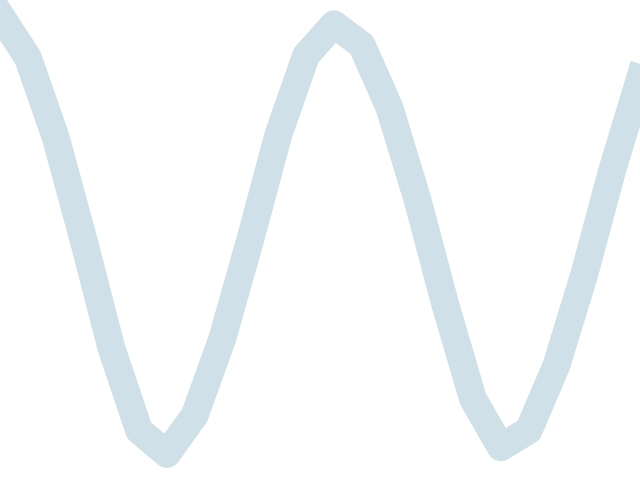
\includegraphics[width=\linewidth,keepaspectratio=true]{plots/2.png}&{\huge\textbf{4}  \hfill }\newline {\tiny{09.12.18 05:00 AM}}\newline\scriptsize{\textbf{}}\newline 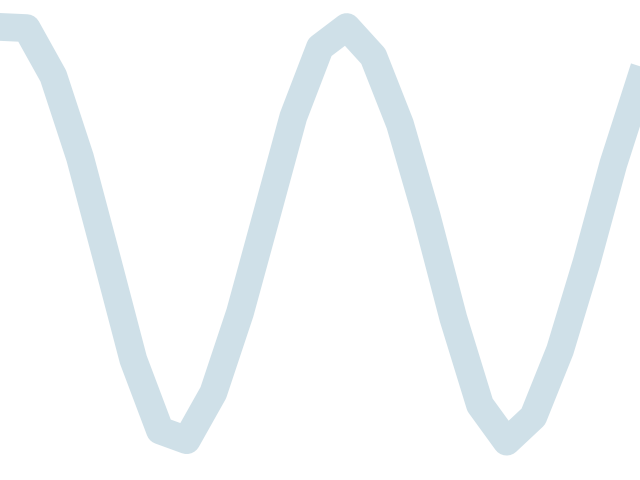
\includegraphics[width=\linewidth,keepaspectratio=true]{plots/3.png}&{\huge\textbf{5}  \hfill }\newline {\tiny{09.13.18 06:00 AM}}\newline\scriptsize{\textbf{}}\newline 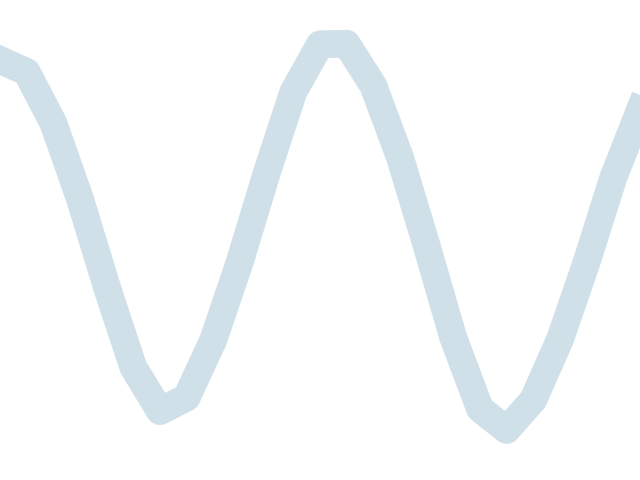
\includegraphics[width=\linewidth,keepaspectratio=true]{plots/4.png}&{\huge\textbf{6}  \hfill }\newline {\tiny{09.14.18 07:00 AM}}\newline\scriptsize{\textbf{}}\newline 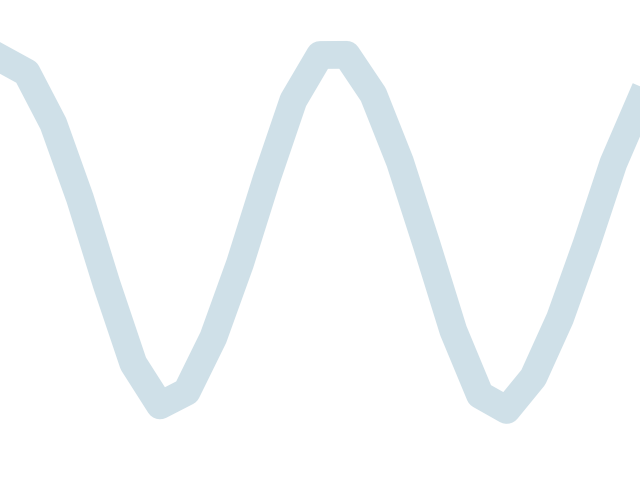
\includegraphics[width=\linewidth,keepaspectratio=true]{plots/5.png}&{\huge\textbf{7}  \hfill }\newline {\tiny{09.15.18 08:00 AM}}\newline\scriptsize{\textbf{}}\newline 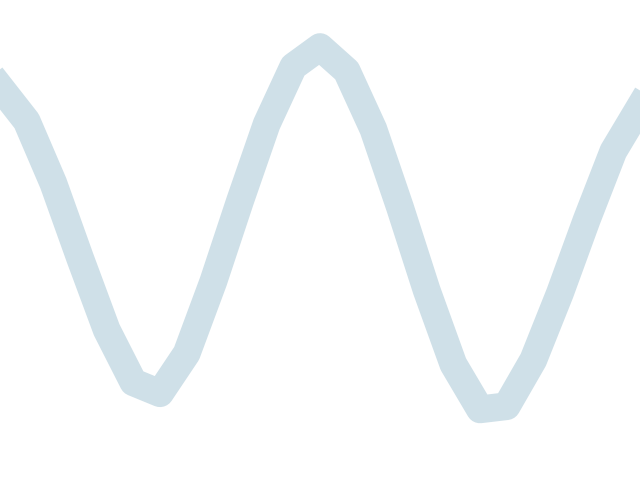
\includegraphics[width=\linewidth,keepaspectratio=true]{plots/6.png}\\\hline {\huge\textbf{8\rule{0pt}{2ex}}  \hfill }\newline {\tiny{09.16.18 09:00 AM}}\newline\scriptsize{\textbf{}}\newline 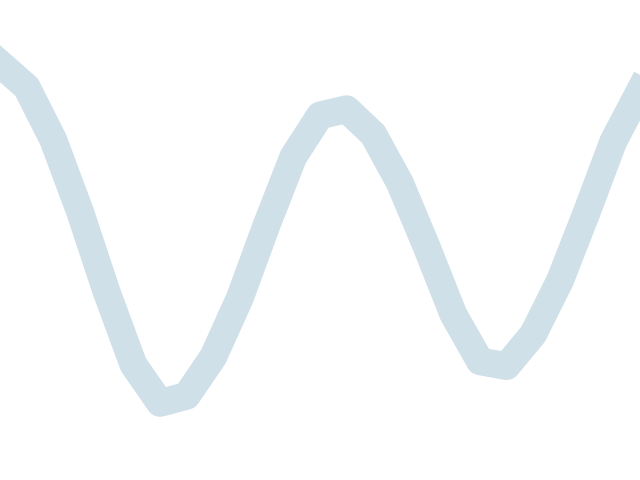
\includegraphics[width=\linewidth,keepaspectratio=true]{plots/7.png}&{\huge\textbf{9}  \hfill \LEFTcircle}\newline {\tiny{09.17.18 10:00 AM}}\newline\scriptsize{\textbf{Yom Kippur\marginnote{\tiny{\textbf{Yom Kippur}\newline\textit{It is customary after reading the Book of Jonah to offer a prayer to all lost mariners.}}}}}\newline 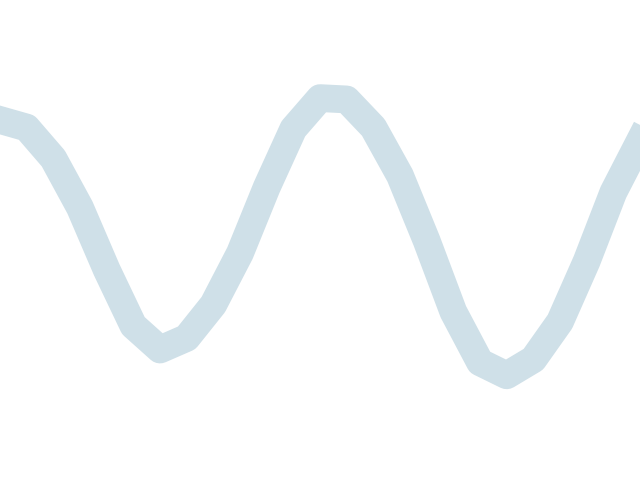
\includegraphics[width=\linewidth,keepaspectratio=true]{plots/8.png}&{\huge\textbf{10}  \hfill }\newline {\tiny{09.18.18 11:00 AM}}\newline\scriptsize{\textbf{}}\newline 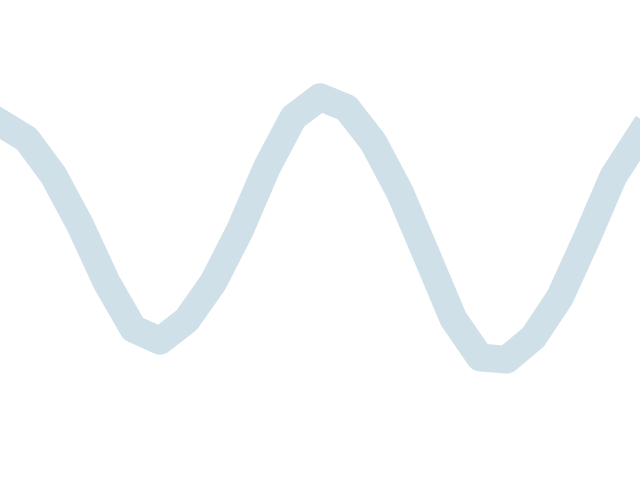
\includegraphics[width=\linewidth,keepaspectratio=true]{plots/9.png}&{\huge\textbf{11}  \hfill }\newline {\tiny{09.19.18 12:00 PM}}\newline\scriptsize{\textbf{}}\newline 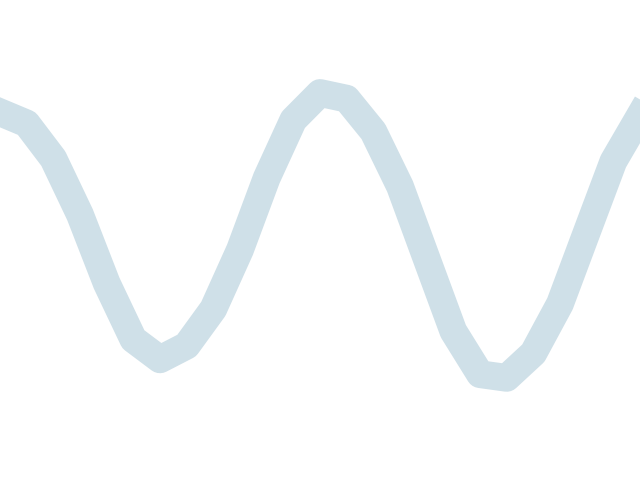
\includegraphics[width=\linewidth,keepaspectratio=true]{plots/10.png}&{\huge\textbf{12}  \hfill }\newline {\tiny{09.20.18 01:00 AM}}\newline\scriptsize{\textbf{}}\newline 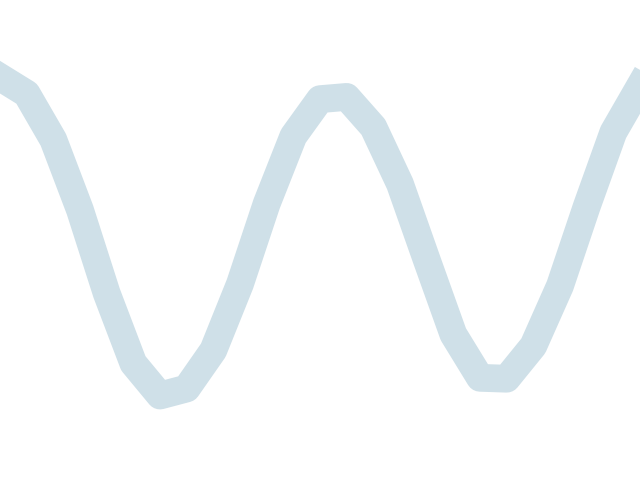
\includegraphics[width=\linewidth,keepaspectratio=true]{plots/11.png}&{\huge\textbf{13}  \hfill }\newline {\tiny{09.21.18 02:00 AM}}\newline\scriptsize{\textbf{}}\newline 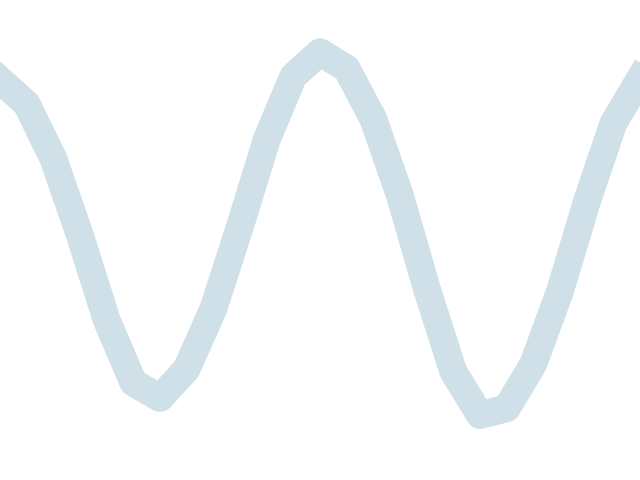
\includegraphics[width=\linewidth,keepaspectratio=true]{plots/12.png}&{\huge\textbf{14}  \hfill }\newline {\tiny{09.22.18 02:00 AM}}\newline\scriptsize{\textbf{}}\newline 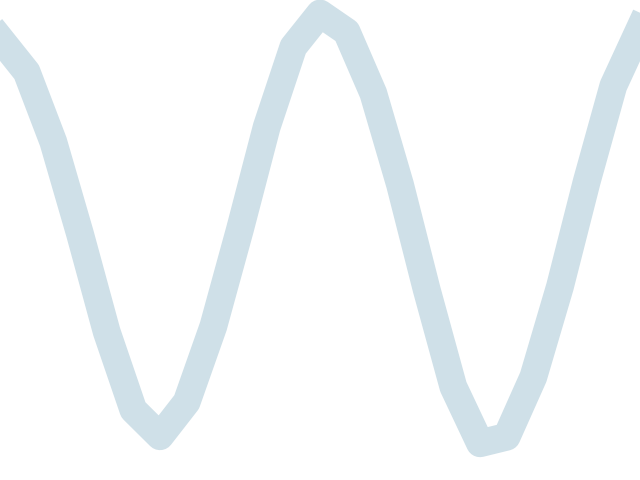
\includegraphics[width=\linewidth,keepaspectratio=true]{plots/13.png}\\\hline {\huge\textbf{15\rule{0pt}{2ex}}  \hfill }\newline {\tiny{09.23.18 03:00 AM}}\newline\scriptsize{\textbf{Sadot begins\marginnote{\tiny{\textbf{Sadot}\newline\textit{Sadat is similar to terrestrial Sukkot, but one is required to build a covered raft rather than a booth. The moon must be visible through the canopy.}}}}}\newline 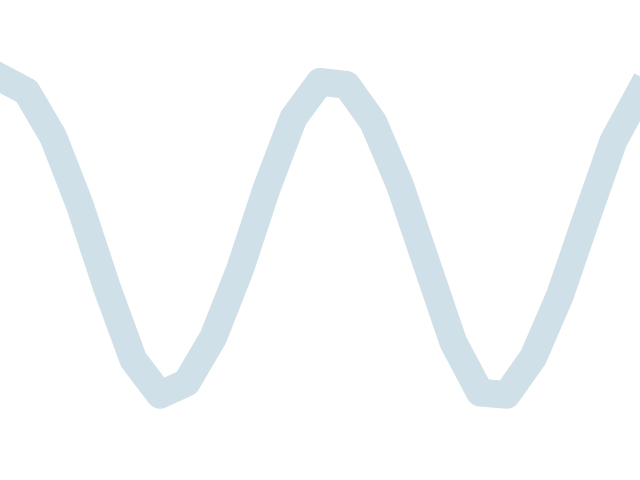
\includegraphics[width=\linewidth,keepaspectratio=true]{plots/14.png}&{\huge\textbf{16}  \hfill \Circle}\newline {\tiny{09.24.18 04:00 AM}}\newline\scriptsize{\textbf{}}\newline 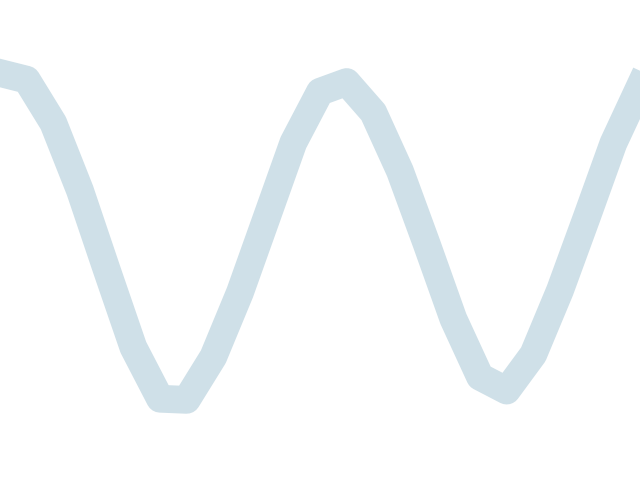
\includegraphics[width=\linewidth,keepaspectratio=true]{plots/15.png}&{\huge\textbf{17}  \hfill }\newline {\tiny{09.25.18 04:00 AM}}\newline\scriptsize{\textbf{}}\newline 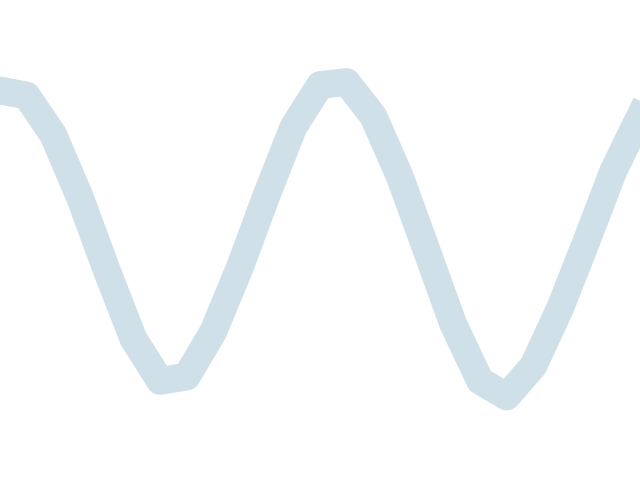
\includegraphics[width=\linewidth,keepaspectratio=true]{plots/16.png}&{\huge\textbf{18}  \hfill }\newline {\tiny{09.26.18 05:00 AM}}\newline\scriptsize{\textbf{}}\newline 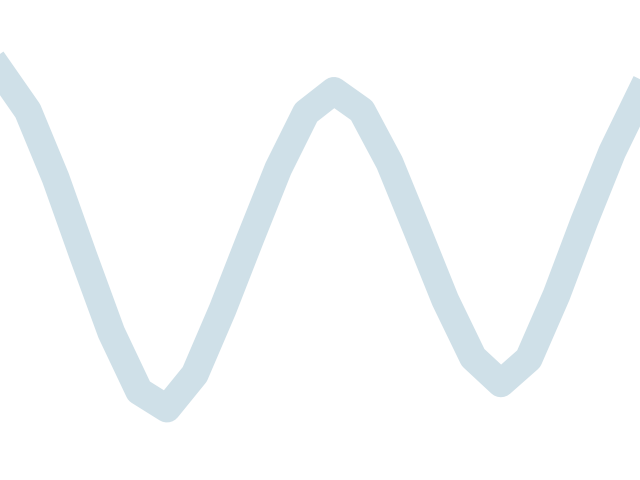
\includegraphics[width=\linewidth,keepaspectratio=true]{plots/17.png}&{\huge\textbf{19}  \hfill }\newline {\tiny{09.27.18 05:00 AM}}\newline\scriptsize{\textbf{}}\newline 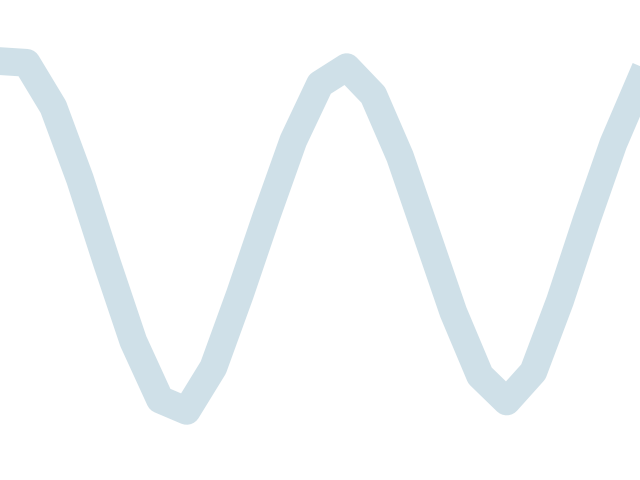
\includegraphics[width=\linewidth,keepaspectratio=true]{plots/18.png}&{\huge\textbf{20}  \hfill }\newline {\tiny{09.28.18 06:00 AM}}\newline\scriptsize{\textbf{}}\newline 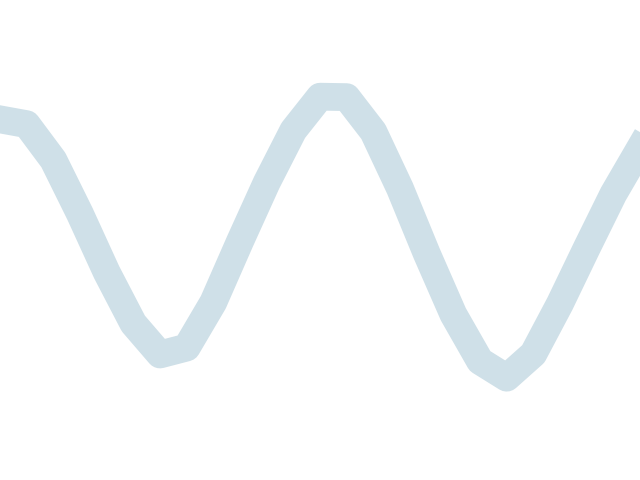
\includegraphics[width=\linewidth,keepaspectratio=true]{plots/19.png}&{\huge\textbf{21}  \hfill }\newline {\tiny{09.29.18 07:00 AM}}\newline\scriptsize{\textbf{}}\newline 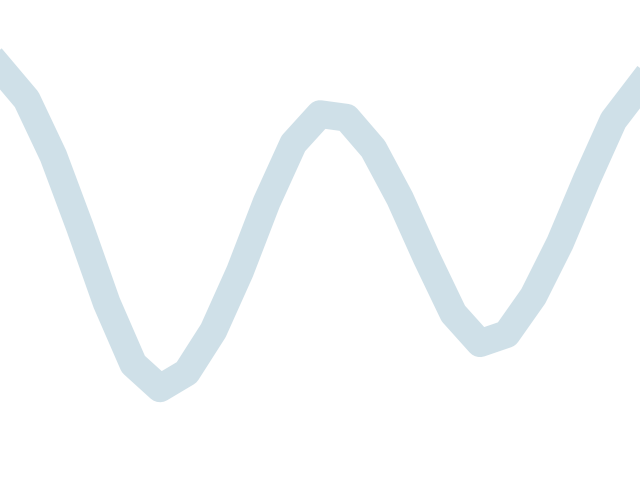
\includegraphics[width=\linewidth,keepaspectratio=true]{plots/20.png}\\\hline {\huge\textbf{22\rule{0pt}{2ex}}  \hfill }\newline {\tiny{09.30.18 08:00 AM}}\newline\scriptsize{\textbf{Sadot ends}}\newline 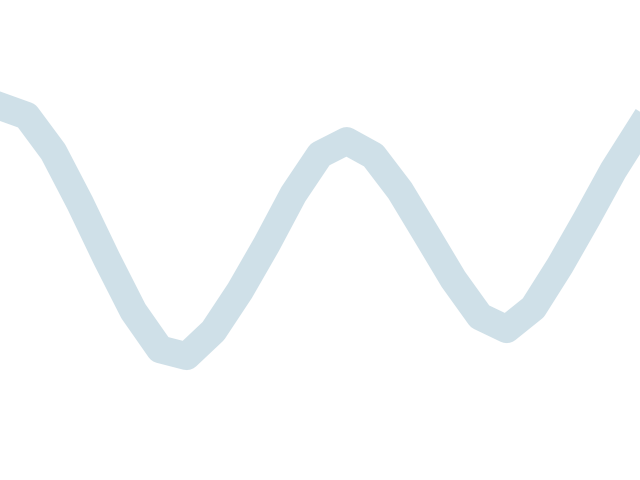
\includegraphics[width=\linewidth,keepaspectratio=true]{plots/21.png}&{\huge\textbf{23}  \hfill \RIGHTcircle}\newline {\tiny{10.01.18 09:00 AM}}\newline\scriptsize{\textbf{Simchat Torah}}\newline 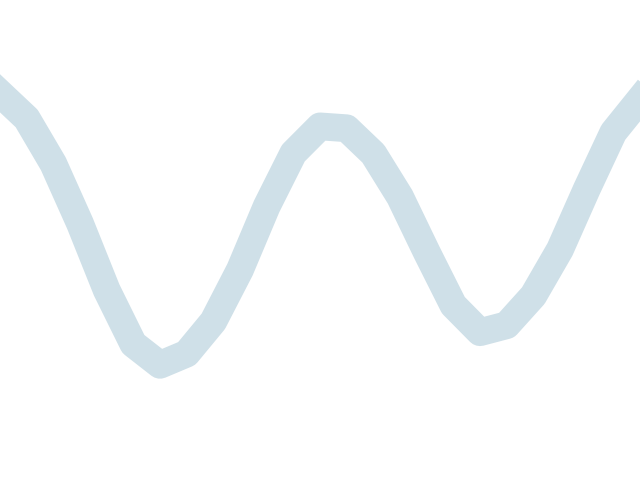
\includegraphics[width=\linewidth,keepaspectratio=true]{plots/22.png}&{\huge\textbf{24}  \hfill }\newline {\tiny{10.02.18 09:00 AM}}\newline\scriptsize{\textbf{}}\newline 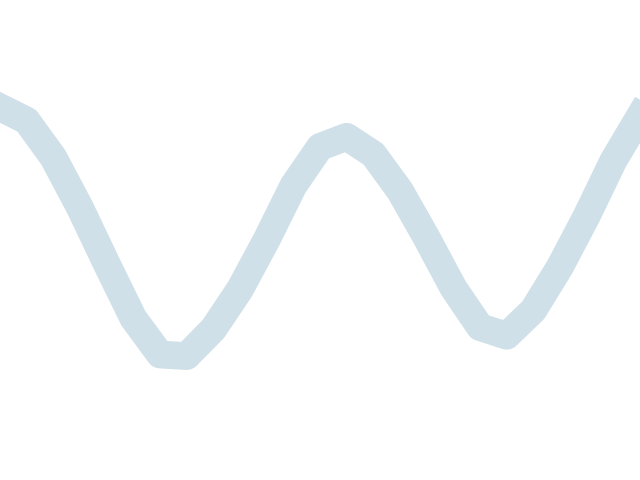
\includegraphics[width=\linewidth,keepaspectratio=true]{plots/23.png}&{\huge\textbf{25}  \hfill }\newline {\tiny{10.03.18 11:00 AM}}\newline\scriptsize{\textbf{}}\newline 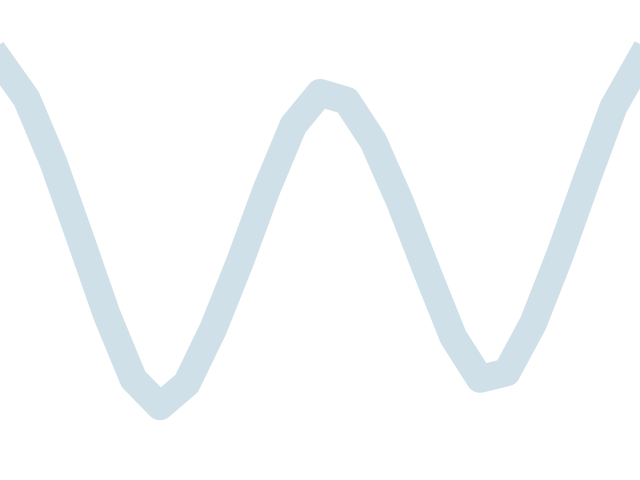
\includegraphics[width=\linewidth,keepaspectratio=true]{plots/24.png}&{\huge\textbf{26}  \hfill }\newline {\tiny{10.05.18 12:00 PM}}\newline\scriptsize{\textbf{}}\newline 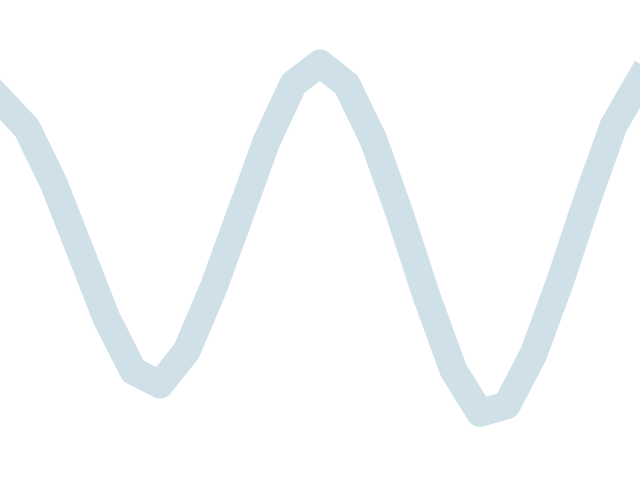
\includegraphics[width=\linewidth,keepaspectratio=true]{plots/25.png}&{\huge\textbf{27}  \hfill }\newline {\tiny{10.06.18 01:00 AM}}\newline\scriptsize{\textbf{}}\newline 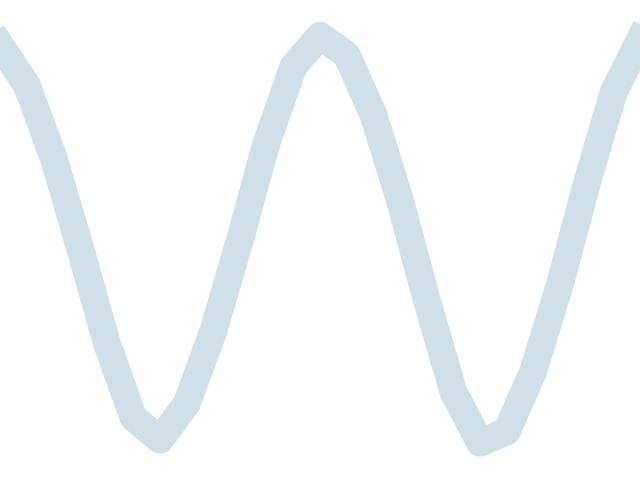
\includegraphics[width=\linewidth,keepaspectratio=true]{plots/26.png}&{\huge\textbf{28}  \hfill }\newline {\tiny{10.07.18 02:00 AM}}\newline\scriptsize{\textbf{}}\newline 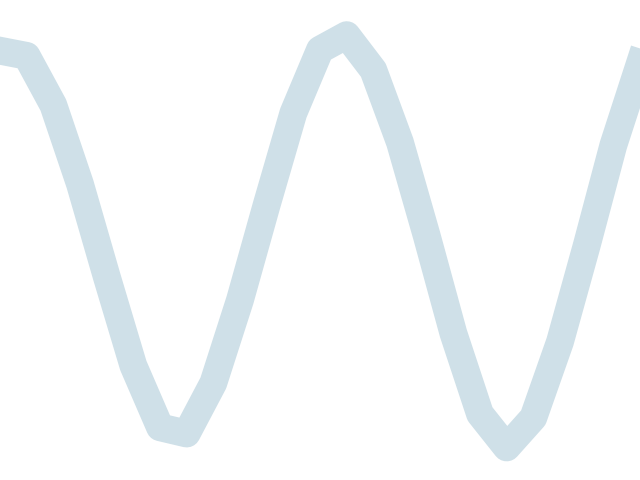
\includegraphics[width=\linewidth,keepaspectratio=true]{plots/27.png}\\\hline {\huge\textbf{29\rule{0pt}{2ex}}  \hfill }\newline {\tiny{10.08.18 03:00 AM}}\newline\scriptsize{\textbf{}}\newline 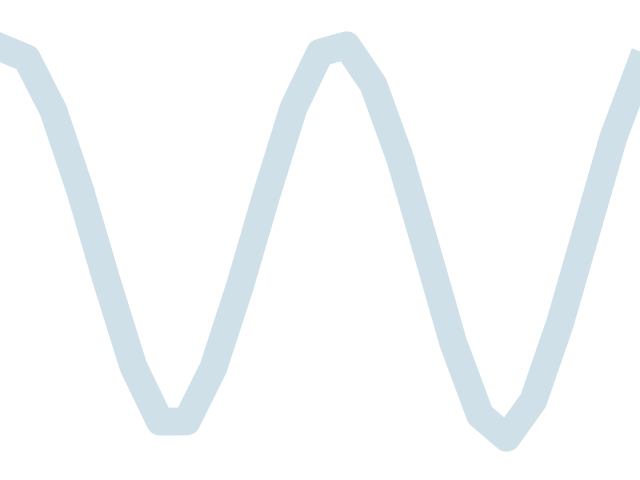
\includegraphics[width=\linewidth,keepaspectratio=true]{plots/28.png}&&&&&&\\\hline\end{tabularx}\end{document}